% Chapter 4

\chapter{Methodology} % Main chapter title

\label{Chapter4} % For referencing the chapter elsewhere, use \ref{Chapter4} 

In this chapter we start with brief overview of related remote attestation schemes in the context of generating offline measurement. After that we present the implementation the ScaRR algorithm to extract checkpoint and list of action as LLVM passes. Checkpoints and list of actions are collected to build offline measurement database that is used for the remote attestation.

\section{Related Attestation Scheme}

\ft{related works in Introduction (As I wrote in my mail, I send it again)}

In this section we present how different attestation scheme encode the offline program representations.

\subsection{C-Flat (2016)}

\ft{no need to make a subsection for each work, just discuss together in a 
single section. You can separate them in paragraphs.}
C-Flat \cite{aberaCFLATControlFlowAttestation2016} is the first remote attestation scheme to detect runtime control flow attack for embedded systems. C-Flat are generating offline measurement by traversing all possible path of program from start node to the termination node. In each node, C-Flat hashes the node ID and the hash of previous node. In the first node, since there is no previous hash, we pass 0. This creates hash chains which is stored as offline measurement database.

\begin{figure}[htbp]
\centerline{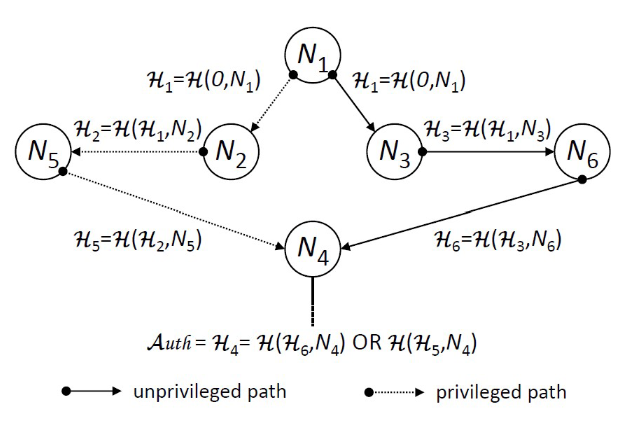
\includegraphics[scale=.5]{Figures/cflat.png}}
\caption{C-Flat}
\label{fig:4-1}
\end{figure}

\subsection{Lo-Fat 2017}

Lo-Fat\cite{dessoukyLOFATLowOverheadControl2017} is improving C-Flat by using hardware support for control flow attestation. Lo-Fat offline program analysis is still inheriting C-Flat approach.

\subsection{Atrium (2017)}

Atrium \cite{zeitouniATRIUMRuntimeAttestation2017} is remote attestation scheme that can provide resiliency against physical memory attack where adversaries can exploit the property of Time of Check Time of Use (TOCTOU) during attestation. In this paper author are describing memory bank attack where adversary can control instruction fetches to benign memory area when attestation is running and direct the fetch to the malicious area otherwise.

\begin{figure}[htbp]
\centerline{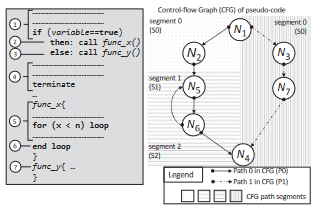
\includegraphics[scale=.5]{Figures/atrium.png}}
\caption{Atrium}
\label{fig:4-2}
\end{figure}

The offline measurement are calculated slightly different compared with C-Flat and Lo-Fat. In Atrium, the verifier perform one-time pre-processing to generate CFG of the program and computes cryptographic hash measurement over the instructions and addresses of basic blocks. C-Flat are only hash the node ID. While this approach can mitigate the TOCTOU attack, the offline measurement generation still grow exponentially as the complexity of the program grow. 

\subsection{LiteHax (2018)}

LiteHax \cite{dessoukyLiteHAXLightweightHardwareassisted2018} is hardware assisted remote attestation scheme that allow verifier to detect these different attacks:

- control-data attack such as code injection or code reuse attack like ROP
- non-control-data attack
- data-only attack such us DOP which do not affect control flow

Different with the previous remote attestation scheme, the offline measurement phase of LiteHax are only generates program CFG without calculating any hash over all control flow and data flow events. However, in the online prover-side verification time, prover are still computing hash and sending it as report to the verifier. Verifier runs symbolic execution and incremental forward data-flow analysis without doing any lookup to offline measurement database.

\subsection{Diat (2019)}

Diat \cite{aberaDIATDataIntegrity2019} is remote attestation scheme that can attest data integrity and control-flow of autonomous systems. To improve efficiency of attestation, the program attested must be decomposed into small interacting modules. Data-flow monitoring is to be setup between critical modules. Control path attestation is being done against novel execution path representation using multiset has (MSH) function \cite{clarkeIncrementalMultisetHash2003}. The use of MSH makes some execution order of the program lost.

\begin{figure}[htbp]
\centerline{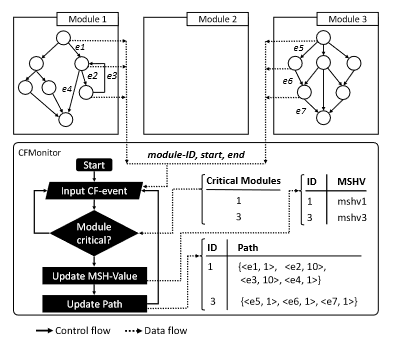
\includegraphics[scale=.5]{Figures/diat.png}}
\caption{Diat}
\label{fig:4-3}
\end{figure}

\subsection{OAT (2019)}

OAT \cite{sunOATAttestingOperation2020} is remote attestation scheme to attest operation integrity of embedded device. OAT defines two type of measurements for control flow attestation: a trace (for recording branches and jumps) and a hash (for encoding returns). These two measurements are encoded as $H = Hash(H \bigoplus RetAddr)$ which called as attestation blob.

\begin{figure}[htbp]
\centerline{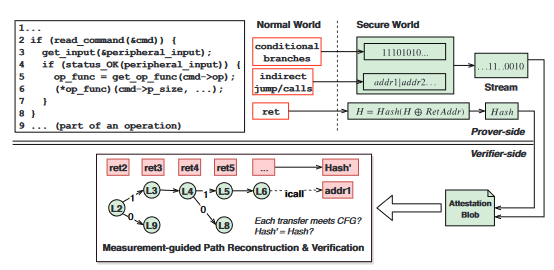
\includegraphics[scale=.5]{Figures/oat.png}}
\caption{OAT}
\label{fig:4-4}
\end{figure}

During verification, verifier reconstruct paths from the attestation blob. The control flow violation is identified when CFI check against an address is failed or mismatched between hash and trace.

Although OAT does not encounter the combinatorial hash explosion in C-Flat, there is a verification overhead since verifier needs to reconstruct the attestation blob. TODO compare the overhead with ScaRR.

\section{ScaRR Control-Flow Model}

ScaRR \cite{toffaliniScaRRScalableRuntime2019} are taking lesson learned from many former runtime remote attestation scheme to build model that can perform in a scalable way and can perform remote attestation on complex system. ScaRR control-flow model consists of two main components, checkpoint and list of action. 

As many previous runtime attestation scheme, ScaRR models and validates the attestion based on program's control flow graph. We need to run one-time measurement computation to extract checkpoints and list of actions of the program.

\subsection{Checkpoints}
Checkpoint is basic block of the program that delimit execution path of the program. ScaRR defines these different checkpoint types:
\begin{itemize}
    \item Thread Beginning: demarcating the start of program/thread
    \item Thread End: demarcating the end of program/thread
    \item Exit Point: representing exit point from application such as system call or out of translation unit function/library call
    \item Virtual-Checkpoint: managing cases for loop or recursion
\end{itemize}

In a program there should be at least Thread Beginning and Thread End checkpoints. Later depends on the structure of the program different checkpoint is marked in the program CFG.

\subsection{List of Actions}

List of actions (LoA) are edges (marked by two checkpoints) that direct one checkpoint to the next one. In program execution path, we only consider edges that identify the unique execution path.

LoA is defined through the following notation:

$$[(BBL_{s1},BBL_{d1}),...,(BBL_{sn},BBL_{dn})]$$

Consider the CFG in the Figure \ref{fig:4-5}. The LoA between node 3 (Checkpoint Virtual) and node 10 (checkpoint ThreadEnd) is  $[(BBL_3, BBL_{10})]$. However, the LoA between node 0 and node 3 is $[]$ (empty set).

\begin{figure}[htbp]
\centerline{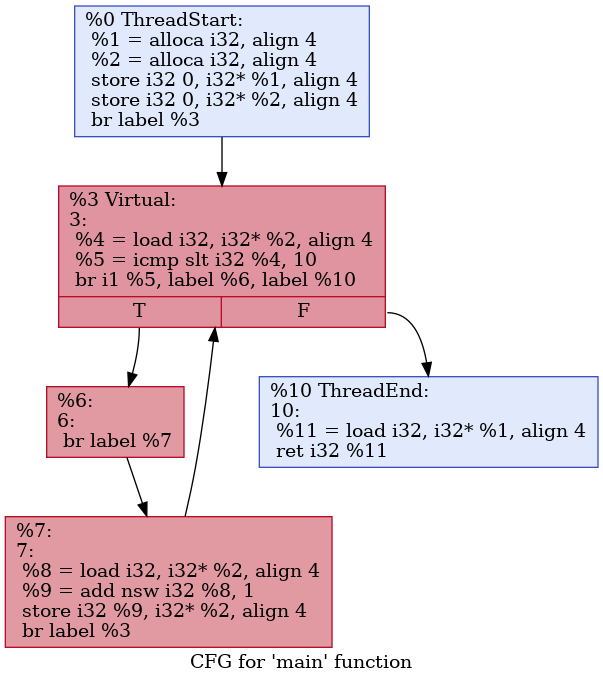
\includegraphics[scale=.5]{Figures/loop-cfg.png}}
\caption{Loop CFG}
\label{fig:4-5}
\end{figure}

\section{Overview}

\ft{I guess we need a section Overview section in which you explain the three 
main ``steps'': Flattening CFG, Find Checkpoints, and last LoA collector. Then, 
you describe how you implemented each part in each section (more or less how 
you already doing).}

\ft{in addition to the pseud code (that are correct btw), you should integrate 
with an image of a CFG that gives an intuition of what you are looking for in 
those passes.}

\section{ScaRR LLVM Pass}
\ft{basically, this is the first part of your methodology section xD}

ScaRR offline measurement is represented as the following key-value pair.

$$(cp_A, cp_B, H(LoA)) \Rightarrow [(BBL_{s1}, BBL_{d1}), ..., (BBL_{sn}, BBL_{dn})]$$

As described in the above, checkpoint is a special basic block that delimit path between execution path in a CFG. $cp_A$ is the start delimiter of the path. $cp_B$ is the end of delimiter. $LoA$ — list of action — is list of significant basic block pairs which define edges 

ScaRR extractor traverses the graph in two passes. The first pass is find whether the basic block is a checkpoint. The second pass traverses the graph and mark List of Action between every two checkpoint. 

\subsection{ScaRR Checkpoint Marker}
\ft{basically, this becomes a section (not subsection). Same for the others.}

The logic of checkpoint marker is to traverse the whole control flow graph at least once. For each basic block, we have to check whether the basic block can be considered as any of checkpoint type mentioned above. To allow marking additional information about ScaRR checkpoint, we are modifying the BasicBlock class to add checkpoint instance variable.

\begin{listing}
\begin{minted}{c++}
    class BasicBlock ... {
    private:
    // add checkpoint field
        Checkpoint cp;

    public:
        // setter and accessor
    void setCheckpoint(Checkpoint);
    Checkpoint getCheckpoint() const;
    ...
    }
\end{minted}
\caption{Add Checkpoint Instance Variable to BasicBlock class.}    
\label{listing:4-1}
\end{listing}

The algorithm to mark the checkpoint is first we iterate all basic block in main function. First we mark the first basic block with no predecessor as ThreadStart checkpoint and basic block with no successor and ThreadEnd checkpoint. 

To identify ExitPoint checkpoint, for each basic block then we iterate  each instruction to find whether any instruction in the basic block is a `call` instruction and has no body defined in this translation unit. Please refer to Listing \ref{listing:4-2}

\begin{listing}
\begin{minted}{c++}
    for (auto &basicBlock: Function) {
        for (auto &instruction : basicBlock) {
            if (isa<CallInst>(i)) {
            auto *call = &cast<CallBase>(i);
            if (call != nullptr && call->getCalledFunction()->empty()) {
                // this basicBlock is ExitPoint
                basicBlock.setCheckpoint(Checkpoint::ExitPoint);
            } 
        }
    } 
\end{minted}
\caption{Finding ExitPoint Checkpoint}    
\label{listing:4-2}
\end{listing}

To mark Virtual checkpoint, we need to find loop header basic block. Although there is no direct API to check whether a basic block is a loop header, LLVM provide it in LoopInfoBase API. See Listing \ref{listing:4-3}

\begin{listing}
\begin{minted}{c++}
    void findVirtualCheckpoint(DominatorTree &DT, Function &F) {
        DT.recalculate(F);
        // generate the LoopInfoBase for the current function
        LoopInfoBase<BasicBlock, Loop>* KLoop = new LoopInfoBase<BasicBlock, Loop>();
        KLoop->releaseMemory();
        KLoop->analyze(DT);
        for (auto &bb : F) {
            // Since the BasicBlock would have been inlined, just traverse from main function
            if (F.getName() == "main") {
            auto loop = KLoop->getLoopFor(&bb);
            if (loop != nullptr) {
                // found VirtualCheckpoint
                        loop->getHeader()->setCheckpoint(Checkpoint::Virtual);
            }
            }
        }
    }
\end{minted}
\caption{Getting Virtual Checkpoint \ft{you could reduce the font size -- also 
for the others.}}    
\label{listing:4-3}
\end{listing}

\subsection{ScaRR LoA Collector}

The algorithm of getting LoA between two checkpoints is little bit more complex. First, we iterate all the basic block and if the basic block is a checkpoint we mark this is $cpA$. Next, we recursively traverse the successor of $cpA$ until we find another checkpoint $cpB$. It is possible for $cpA = cpB$. If there is no branch between the two checkpoint, the LoA is an empty set. If there is a branch, the first LoA is always be $cpA$ and the second LoA is always be the first basic block after the branch \textemdash{} which can be $cpB$ or just non checkpoint basic block. Interested readers can refer to the implementation of this pass to see the detail.

\subsection{Running The Pass}

To mark the list of Checkpoints, we can invoke LLVM \texttt{opt} as follow.

\begin{listing}
\begin{minted}{c++}
    opt -passes=scarr-cp-marker <file>.ll
\end{minted}
\caption{Mark Checkpoint in BasicBlock}    
\label{listing:4-4}
\end{listing}

We can see the basic blocks output that has been marked with checkpoint using LLVM dot-cfg pass.

\begin{listing}
\begin{minted}{c++}
    opt -passes=scarr-cp-marker,dot-cfg <file>.ll
\end{minted}
\caption{Print Checkpoints in CFG dot file}    
\label{listing:4-5}
\end{listing}

The commands above generates different dot files per function. We can use xdot command line from graphiz to see the graph. 

To mark the list of actions between checkpoints, we can invoke LLVM \texttt{opt} as shown in Listing \ref{listing:4-6}

\begin{listing}
\begin{minted}{c++}
    opt -passes=scarr-cp-marker,scarr-loa-collector <file>.ll
\end{minted}
\caption{Get List of Actions}    
\label{listing:4-6}
\end{listing}

Note that we have to run scarr-cp-marker before scarr-loa-collector.

The result and its interpretation are discussed in the next chapter.